\documentclass[border=10pt]{standalone}
\usepackage{tkz-euclide}

\usepackage{tikz}
\usetikzlibrary{calc}

\begin{document}

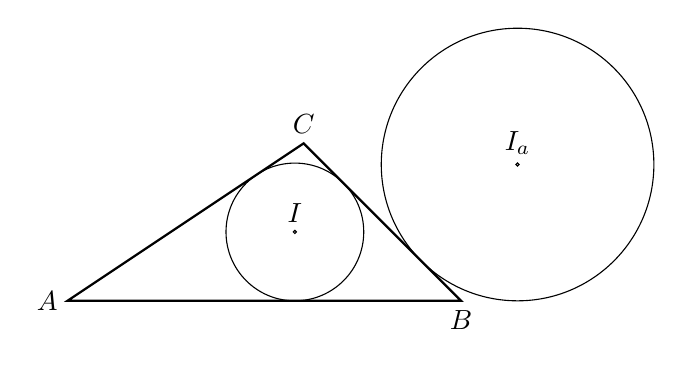
\begin{tikzpicture}
    % Koordinaten der Eckpunkte des Dreiecks
    \coordinate [label=left:$A$] (A) at (0,0);
    \coordinate [label=below:$B$] (B) at (5,0);
    \coordinate [label=above:$C$] (C) at (3,2);

    % Zeichne das Dreieck
    \draw[thick] (A) -- (B) -- (C) -- cycle;

    % Berechne Seitenlängen
    \pgfmathsetmacro{\a}{8^(1/2)}
    \pgfmathsetmacro{\b}{13^(1/2)}
    \pgfmathsetmacro{\c}{5}

    % halber Umfang
    \pgfmathsetmacro{\s}{(\a + \b + \c) / 2}
    % Fläche des Dreiecks
    \pgfmathsetmacro{\A}{5}
    % Inkreisradius
    \pgfmathsetmacro{\rho}{\A / \s}
    % Ankreisradius
    \pgfmathsetmacro{\rhoa}{\A / (\s - \a)}
    % Alpha halbe
    

    % Zeichne den Inkreis
    \coordinate [label=above:$I$] (I) at (\s-\a,\rho);
    \draw (I) circle (0.2mm);
    \draw (I) circle (\rho);

    % Zeichne den Ankreis a
    \coordinate [label=above:$I_a$] (Ia) at (3*\s-\c-\b-\a, \rhoa);
    \draw (Ia) circle (0.2mm);
    \draw (Ia) circle (\rhoa);

    % Zeichne Winkelhalbierende alpha
    %\draw (0,0) -- ()

   
\end{tikzpicture}

\end{document}